%thesis.tex 
%Model LaTeX file for Ph.D. thesis at the 
%School of Mathematics, University of Edinburgh

\title{Fairness in Multilingual NLP}
\author{Seraphina Goldfarb-Tarrant}
\date{2023}

\documentclass[phd,ilcc,oneside,leftchapter,parskip]{infthesis}

\usepackage[T2A,T1]{fontenc}
\usepackage[utf8x]{inputenc}

\usepackage[english]{babel}

\usepackage{natbib}

% \usepackage{biblatex}
% \addbibresource{biblatex_bib.bib}

\usepackage{latexsym}
\usepackage{graphicx}
\usepackage{amsmath}
\usepackage{wrapfig}
\usepackage{times}

\usepackage[dvipsnames]{xcolor}

\usepackage{subcaption}
\usepackage{mwe}
\usepackage{booktabs} % Top and bottom rules for tables
\usepackage{svrsymbols}

\usepackage{tikz-dependency}
\usepackage{tikz-qtree}
\usepackage{paralist}
\usepackage{tikz}
\usetikzlibrary{shapes,arrows,positioning}
\usetikzlibrary{matrix}
\usepackage{etoolbox}
\usepackage{bm}
\usepackage{amssymb}
\usepackage{amsfonts}
\usepackage{amsmath}
\usepackage{csquotes}
\usepackage{verbatim}
% \usepackage{todonotes}

\usepackage{epigraph}
\setlength{\epigraphwidth}{0.7\textwidth} 

\usepackage[final]{pdfpages}

\usepackage{url}
\usepackage{hyperref}
\usepackage{cleveref}
\urlstyle{rm}
\definecolor{revcolor}{rgb}{0.81, 0.09, 0.13}
\definecolor{darkblue}{rgb}{0.2, 0.2, 0.6}

\hypersetup{
    colorlinks,
    citecolor=darkblue,
    filecolor=black,
    linkcolor=darkblue,
    urlcolor=darkblue
}

% \usepackage{lsubfiles}

\newcommand{\E}{\mathbb{E}}


\abstract{TLDR}

\begin{document}

%% First, the preliminary pages
\begin{preliminary}

%% This creates the title page
\maketitle


\begin{laysummary}
Laysummary
\end{laysummary}

% Acknowledgements
\begin{acknowledgements}
ACK


\end{acknowledgements}


%% Next we need to have the declaration.
\standarddeclaration

\dedication{}

%% Finally, a dedication (this is optional -- uncomment the following line if
%% you want one).
% \dedication{To my mum
%% Create the table of contents
\tableofcontents

%% If you want a list of figures or tables, uncomment the appropriate line(s)
% \listoffigures
% \listoftables

\end{preliminary}

% %!TEX root = ../thesis.tex
\chapter{Introduction} 
\label{chapter:introduction}
In the past decade, Natural Language Processing (NLP) systems have come to saturate everyday life. NLP has expanded from being used to translate webpages and recommend new videos to having inescapable reach. It is now also used to moderate social media content \citep{ofcom_content_mod}, where all posts are filtered through an NLP system that judges them as hateful/not-hateful, acceptable/not-acceptable, and either removes or suppresses the sharing of posts that fail this check. NLP is used to generate answers to any user questions about any topic \citep{rajpurkar-etal-2016-squad, rajpurkar-etal-2018-know}, by sifting through millions of documents and determining which ones are relevant and worth knowing about and presenting those, discarding others. It is used to  track public opinion about products or politicians \citep{peoples-2020-modeling}, by analysing the sentiment of all of the information said about them online. NLP is used to sort and filter resumes for potential new workers \citep{parasurama-sedoc-2022-gendered}, by comparing each new resume to previous successful hires for a job, and flagging which ones to send to a phone-screen and which ones to reject. It is also used to later fire those same workers \citep{forbes_hiring}, by reading data about their productivity and predicting who shouldn't make the cut. These examples are a small set of the myriad applications that use NLP today, chosen as the areas the are directly relevant to the research in this thesis. There are so many more; most people in the UK and US come into contact with NLP or AI multiple times daily, though many of them are not aware of it \citep{kennedy2023public}.

This increase in scope and usage of NLP systems comes with many promises of efficiency, cost reduction, and even social good. For all of the uses above, there are bright promises. NLP for content moderation on social media can reduce hatespeech and aggression online, which has reached a volume and velocity that is completely unmanageable for human moderators. When left unchecked, it is linked to amplification of violence in the real world. NLP for retrieval and question answering can enable greater and easier access to information, a necessary step in searching and organising the vast quantities of digital information and democratising information access. NLP as sentiment analysis of public opinion can enable direct and inexpensive democratic feedback for companies or policies; direct feedback that might otherwise be too logistically challenging and expensive to gather. NLP in hiring systems could enable processing more applications, which could give a broader segment of the population a chance, and create systems that are less dependent on `who you know' and on the instincts of a few HR representatives tasked with reading through a resume slush pile.

But this territorial expansion introduces many new harms that diminish these promises.  
The often referenced promise of mathematical objectivity---freeing us from human subjectivity, inconsistency, and biases---has proven to be mythical. 
At best, NLP systems learn and propagate these same biases, but with a veneer of objectivity that fosters over-reliance \citep{oneil2016weapons} and reduces accountability and recourse when data is incorrect and decisions go wrong. 

A large and growing body of work analysing NLP systems has shown that they do not behave similarly and work equally well for different genders, races, nationalities, and other demographic groups. This disparate performance across demographics is the standard definition of \textbf{fairness}, which we use throughout this thesis: these systems are not \textbf{fair}. 
So given that NLP systems, and the data, models, and optimisation and evaluation metrics they are composed of are \textit{not} inherently fair, we must analyse the ways they are not, so we know what to expect and can mitigate where possible. When NLP systems are not fair, companies and organisations using them (and people subjected to their outputs) are worse off than before automation systems, since this flawed system has now been scaled. An individual Human Resources manager may have flaws and biases, but they work for only one or a few companies and have time to read only so many resumes in a day. Some resumes will be sent to a different person, who may have different biases, preventing the inequities of the first person's views from being complete and consistent over a wide swath of potential jobs. When a flawed and biased NLP HR system is scaled, it does not sleep, get tired, or clock-off and can process as many thousands of resumes as time and compute allows. The same system is used by many companies. The very variability of human behaviour, and the inconsistencies in human decisionmaking that are often considered undesirable, limit the possible scope of each individual's (or even each company or organisation's) biases. This lack of scaling of humans is an accidental safeguard. An NLP system, in contrast, replicates the same biases to an unlimited extent, and whatever unfortunate minorities it is biased against will experience more widespread discrimination. This is the situation of the present day, and sets the scene for this research.

The research world noticed this, eventually. Fairness problems in NLP started to become well-known in the NLP community in 2016, as NLP itself began to directly touch more lives and have more impact \citep{hovy-spruit-2016-social}. Attention in the research world, and the public, has grown exponentially since\footnote{\url{https://fairmlclass.github.io/1.html\#/4}}. By the time of writing, major conferences now have a dedicated track for fairness research\footnote{\url{https://aclrollingreview.org/cfp}}, encourage papers to self-declare potential hazards\footnote{Section A2 in \url{https://aclrollingreview.org/responsibleNLPresearch/}, and section 1c in \url{https://neurips.cc/Conferences/2021/PaperInformation/PaperChecklist}}, and have an ethics committee appointed to review potential fairness problems in any work\footnote{\url{https://www.aclweb.org/adminwiki/index.php?title=Formation_of_the_ACL_Ethics_Committee}}. Yet despite all the attention and effort expended on fairness in NLP, we as a community have made only such a small dent in known problems as to now be aware of the magnitude of still unaddressed fairness problems. Both discovering and addressing fairness problems in an NLP system remains extremely challenging. 

There are a couple of reasons for this challenge, which have prevented the community from making a larger dent. One of the most salient ones is that NLP systems today are complex; they involve multiple stages of model training, as is the case with Transfer Learning (discussed and defined in \S\ref{sec:bg_transfer_learning}). How to measure and mitigate unfairness in a multi-part NLP system is not clear, and systems are now always multi-part. How does a measurement or mitigation at one stage relate to the other stages? What can be trusted to hold across stages? This thesis attempts to take a step towards remedying this. It asserts, throughout each of the sections, that you cannot study just one part of an NLP system in isolation, without first understanding how it affects the other parts. 

There is real difficulty in even defining unfairness, and a substantial percentage of fairness papers neglect to define it at all \citep{blodgett-etal-2020-language, goldfarb-tarrant-etal-2023-prompt}. There are multiple ways that a system can be unfair. NLP systems are often not \textbf{allocationally fair}; they and have different accuracies and rates of false positives and false negatives for different demographics. A example such situation is when a toxicity detection system has much higher rates of false positives for text that is actually neutral or positive but contains terms about race, religion, or sexual orientation. In such as case, a sentence like \textit{I am a gay man} can be flagged as toxic and censored, as was the case with Google's toxicity detection system in 2018 \citep{Dixon2018MeasuringAM}. NLP systems are also often not \textbf{representationally fair}; they reproduce and propagate negative stereotypes for minoritised demographics \citep{crawford_keynote}. For example, prominent generation systems will disproportionately describe women as taking carer roles, and portray racial minorities as criminals \citep{sheng-etal-2019-woman}. 

There is not even a consensus on how best to measure each type of unfairness. Most metrics used to measure fairness are ad-hoc and have not been standardised or analysed for \textbf{predictive validity}---their ability to predict actual fairness problems that will occur--or \textbf{concurrent validity}---their agreement with other metrics in use. If you cannot measure something, `your knowledge is of a meagre and unsatisfactory kind' \citep{kelvin1891popular} and you cannot know whether any improvements you make actually worked. So we begin by making some progress towards assessing predictive and concurrent validity of fairness metrics in Part~\ref{part:measurement}.  

Another challenge is that fairness issues can appear at almost any stage of building an NLP system \citep{suresh2021framework}, and as mentioned, the relationship between the stages is poorly understood. NLP papers commonly claim that `model biases reflect biases in data they were trained on'\footnote{This refrain is ubiquitous, and is apparently even the rationale that ChatGPT gives: \textit{Yes, language models can have biases, because the training data reflects the biases present in society from which that data was collected.} as reported in \url{https://news.mit.edu/2023/large-language-models-are-biased-can-logic-help-save-them-0303}} 
but this is such a gross oversimplification as to be both unhelpful and misleading. It glosses over questions such as: \textit{how did the biases get into the data? Do imbalances in labels over different sensitive groups count, or do only stereotypes count?} And it glosses over all the other causes, of which there are seven high level kinds in \citet{suresh2021framework}, and some additional in other works \citep{mehrabi_survey}. I expect the prevalence of this statement is a way of shirking responsibility. If it is the data's fault for being biased, and society's fault for creating biased data, then it is not the fault of the engineer or company for creating a biased model. It's just the world we live in. 

But it is not the world we live in. It is the world we are making. All choices in the process of training an NLP model can affect the resulting bias. A resume filtering system can be trained on data in which humans made racist or sexist decisions -- say in the past they didn't hire non-men, or non-white, or only hired young people or people who went to certain schools. This is \textbf{historical} bias, and that bias in the training data will not only persist, but be amplified, an effect which is much less frequently discussed but is common \citep{zhao-etal-2017-men, jia-etal-2020-mitigating, cabello-etal-2023-evaluating, pmlr-v80-hashimoto18a}. 
%This already weakens the ability to shirk responsibility for a system that not only reflects existing societal biases, but increases them . 
Then this system, which is already dubiously `only reflecting training data' will scale, with the authority of an objective AI system behind it. This happened with Amazon's attempt at an AI for Human Resources, which would not hire women at all because, historically, Amazon had not hired very many of them.\footnote{\url{https://www.reuters.com/article/us-amazon-com-jobs-automation-insight-idUSKCN1MK08G}.} There are also \textbf{sampling}, aka \textbf{representation}, biases. For instance, a content moderation and toxicity detection system can be unfamiliar with non-prestige dialects and censor them incorrectly, as happened when tweets in African-American Vernacular English (AAVE) were incorrectly flagged as toxic speech \citep{sap-etal-2019-risk}. Even though AAVE is common in the \textit{world}, it was not well-represented in data the model has seen. So even within dataset biases, there are multiple kinds with different reasons behind them. There are other sources beyond dataset biases. The above example of historical bias in hiring is actually an example of another type of bias as well, \textbf{measurement} bias. This NLP resume filtering system uses labelled data for supervised learning (as is quite common) where the labels are a proxy for the task that is to be learnt -- e.g. \textit{was previously hired based on this resume} is a proxy for \textit{was suitable for the job}. That label can be a better or worse proxy for the desired task. This gap between the thing being measured and the unmeasurable quantity of interest is \textbf{measurement} bias. These are only a few of the many ways that unfairness can enter a system, selected as examples as they are the types that I spend the most time examining below. There are more subtle ways that can make mitigation even more challenging, which I discuss in Part~\ref{chapter:background}.

% Remining things are aggregation (example from hardt) and evaluation (maybe example from my reality check paper) and also learning (the metric being optimised). 

%Fairness issues can arise also in fitting the same function to multiple groups that require different functions (aggregation bias) and in the metric used to evaluate (evaluation bias) \citep{hardt2016equality}.


%it has become a vital responsibilty for us as researchers to examine our models, algorithms, and data as to their behaviour for different demographic groups. Do they behave similarly and work equally well for different genders, different races, different nationalities? We need to know this information to ensure that the systems we build innovate, and improve society, rather than accelerating marginalisation and societal divisions and isolation. 

%These are the ways that unfairness can enter a system. 

%PICK UP HERE -- connect to the issues of *scaling* and of *not knowing how something gets into the system. Might need to connect transfer learning to it more smoothly -- since transfer learning is responsible for scale, and basically introduces a new source of all of these types of biases that is unexplored (a second set of data and of sampling and of measurement blah blah). It is also now the dominant paradigm (scale) that has been underexplored. And we want to know if these systems are better or worse than systems before using them, and we also want to pinpoint the source to enable us to mitigate it -- if we performed mitigation at the wrong stage it might not work

An NLP system can contain one, many, or all of these sources of bias, and this bias can enter in via the data collection, dataset splits, learning objective, model architecture, model deployment choices (such as decoding hyperparameters or classifier thresholds). And most of these choices are now made \textit{twice} or more. Current scale in NLP is driven by \textbf{transfer learning}, where a model is trained on high resource task(s) or language(s) (e.g. unstructured web crawl text) and then ported to a lower resourced one (e.g. any supervised task requiring labels, like sentiment analysis) -- not necessarily objectively \textit{low resource}, but relatively lower resourced, i.e. with less data than the dominant task or language being used for transfer. 
%Within a language, this is usually done with a language model pre-trained on large scale web text and then applied to a supervised learning task requiring labelled data. Between languages, this is usually done between English and another language with less or no labelled data. 
It was already difficult to pinpoint where biases enter a system, and with transfer learning most systems are composed of multiple sets of training data, multiple objectives, multiple measurements. 
%The little work on existing multi-part systems shows that individually fair components are not necessarily fair under composition \citep{dwork2018group}

Transfer learning is now the dominant paradigm in NLP, but previous to the work in this thesis, fairness research considered only one of the two stages: the pre-training or the fine-tuning stage. If a language model that will later be used in our example resume filtering system (which we refer to as an \textbf{upstream model}) has been debiased with regard to gender, will the classifier on top of it (which we refer to as the \textbf{downstream model}) also be debiased, or not? If instead the classifier is debiased, is the language model also safe to use, or will bias then surface if the language model is used in another task, or directly without the classifier? We cannot answer these questions without studying the entire system and learning the relationship between upstream and downstream models. And without these answers,
%further complicating this already multiplex ecosystem of threats to fairness. It is now even harder to track and mitigate biases in NLP systems because they are multi-stage. 
bias mitigation methods or measurements are at best ineffective, and at worst misleading. With these answers we can apply effective bias mitigation strategies at the correct stage of the system, and we will understand the contribution of transfer learning to fairness in NLP systems and be informed as to whether systems are becoming better or worse as they scale. This understanding is a pre-requisite to effective work in NLP bias, and yet before the work in this thesis, the field had little knowledge of it.

So here, in the below, we explore a previously yet unstudied area of NLP fairness; how unfairness, having entered a system, persists and travels throughout it. 

We first focus, in Part~\ref{part:measurement}, on fairness measurement at different stages of transfer learning. No real research can be done without good measures, and we need an understanding of how measures of bias relate at different stages of transfer learning, since interventions are customarily applied at one stage. In Chapter~\ref{chapter:intrinsic_bias_metrics}, we study whether the most common \textbf{intrinsic} bias measurements--at the language model pre-training stage--are predictive of later downstream, or \textbf{extrinsic}, bias in two classification tasks in two languages. We find that they are not predictive, and that the widespread use of these measures has been leading to a false sense of progress in debiasing research. Most work was at the time done on only upstream models, and our work shows that we cannot tell whether debiasing efforts are propagating downstream. Our results show that more effort needs to be spent on measuring bias on the downstream task itself. Following this, in Chapter~\ref{chapter:gender_bias_probing}, we study the relationship of transfer learning measurements in the \textit{reverse} direction. Here we ask how a pre-trained upstream language model changes when different debiasing methods are applied downstream. We find that a new metric, based on information theoretic probing (also known as minimum description length (MDL) probing) \citep{voita-titov-2020-information} can, when applied to the pre-trained language model, differentiate between different downstream bias levels, and different downstream debiasing techniques, and show which are more effective. We find that this measure is predictive of how robust debiasing of the pre-trained language model is, and whether the debiasing will remain if that model is then used in another task. These two results together imply that the \textbf{geometry} (cosine or other distance measures, previously used as upstream metrics) of concepts in language model representation space does not reliably predict downstream bias, but the \textbf{extractability} of concepts (as measured by information theoretic codelengths) is better predictor. In that work, we also are the first to use a wide suite of ten downstream fairness metrics that refer to slightly different notions of fairness. We find that though they tend to track together, if we had naively used a subset of them, based on what was most popular for certain datasets, we might have come to a different conclusion. Different metrics are suitable for different applications and scenarios, and they do not always tell the same story. 

% Prior to the work in this dissertation, it has been unknown how fairness (and lack of) in an initial model relates to fairness in a system in which it is used. 

We then use our findings on measurement to conduct experiments addressing a broad question about how the use of transfer learning affects the fairness of a system. There is no previous work on this, but previous work on aspects of transfer learning leads to two competing possibilities of how transfer learning could impact fairness. Does transfer learning \textit{improve} fairness, because the additional data sources lead to overall better models that are better at modelling long tail phenomena (and data on minorities is often long tail)? Or does the additional complexity bring in new or magnified undesirable biases, via one of the many mechanisms introduced above? 
%We study this for transfer learning between tasks within one language, and also for transfer learning between different languages. Within one language, will a language model that has been trained on raw text data that underrepresents women in prestige careers in STEM also fail to appropriately classify women's biographies into STEM roles \citep{biosbias} and incorrectly filter women's resumes for STEM positions? 

In Part~\ref{part:crosslingual} we pick a task---sentiment analysis, which we selected since this task enables us to test in a number of languages---and study this effect for transfer learning between \textit{tasks/objectives} (the current dominant NLP paradigm, which we will sometimes refer to as monolingual transfer learning to distinguish it) and transfer learning between \textit{languages}, called multilingual or crosslingual transfer learning (used interchangeably but the field and by us). Prior to our first investigation, previous work had shown that language models trained on unstructured text have gender and racial biases \citep{bolukbasi, Caliskan2017SemanticsDA, zhao-etal-2019-gender, zhao-etal-2020-gender, sheng-etal-2019-woman}. So we asked, will this carry through in monolingual transfer learning and cause gender and racial biases to appear or increase in a downstream sentiment model, beyond what can be attributed to the downstream training data? For instance, let's say that an upstream language model has learnt to associate conventionally negative attributes with certain minorities, such as to represent gay men as doing drugs, and black men as pimps (examples from \citet{sheng-etal-2019-woman}). Will a sentiment classifier built on this upstream language model also associate negative sentiment with gay and black men, \textit{even if} there is little or no data about gay and black men in the sentiment training data? 
Or will that bias be overridden or lost, either because the role of the classifier is strong enough to disregard that, or because the now larger and more expressive system can generalise better to other positive association involving black and gay men, such as stars in politics and arts, or affirmational personal stories, such as those in \cite{Dixon2018MeasuringAM}? We find that, overall, the additional stability from transfer learning is helpful in a resource constrained setting (i.e. one in which you cannot gather more annotated sentiment data), and this effect is enough to reduce overall gender and racial biases (despite new negative associations having been introduced).

We also study this effect for transfer learning between languages, or \textbf{cross-lingual transfer learning}. In this setting, not only can an upstream model learn biases from multiple data sources, but also from multiple languages. Exactly how much information cross-lingual transfer learning shares across languages is not well understood and there are some contradictory empirical studies \citep{conneau-etal-2020-unsupervised, artetxe-etal-2020-cross}.
We ask, in cross-lingual transfer learning, if a language model has learnt harmful stereotypes in one language, can those negative associations carry across languages? In the above example where a model has learnt negative associations \textit{in English} about black and gay men, will a classifier in Japanese have these same associations, if they do not occur in Japanese? Can the collision between competing stereotypes in different languages weaken them, and in effect fight bias with bias? \citep{stanovsky-etal-2019-evaluating}. Can anything be done in the initial task before transfer, to ensure better outcomes in the second task? We find that, contrary to what we found in monolingual transfer learning, cross-lingual transfer learning tends to (with exceptions) exacerbate biases, though this effect can be mitigated with distilled/compressed models with little loss in performance. 

In Part \ref{part:generation}, we look at a third type of system: retrieval augmented generation, which presents an inversion of the standard transfer learning setup. In the standard setup,  a language model feeds into a classifier, and in retrieval augmented generation, the classifier selects source documents to answer a query, and this feeds into a language model, which conditions on those documents to generate an answer. This inverted system allows us to also ask the reverse question: if a language model has learnt problematic associations and stereotypes, can these be counteracted by conditioning on source documents? For instance, if a language model generates results about women predominantly in low-prestige roles, will it change this if it is conditioned on source documents about female CEOs and doctors? Or is it more likely to ignore the source information in this case then in the case of male CEOs and doctors? Or, as a third option, the retriever itself is biased, and doesn't select documents about female CEOs, so we never even get to that point?

However, prior to our work, not only was there no research examining how fairness flows between retrieval models and generative language models, there was little research analysing neural retrievers at all. So we began by asking the sub-question, inspired by all our work in Parts~\ref{part:measurement} and \ref{part:crosslingual}: a retriever representation is necessarily a compression of a document, so what information is actually in this representation, such that 
 a language model can condition on it? (Recall Chapter~\ref{chapter:gender_bias_probing} where information in a representation as measured by information theoretic probing is most predictive of bias). Is information about demographics--gender, race, etc--in a retriever representation predictive of allocational bias in retrieved results? That is, does a retriever with stronger information about gender pick documents about gender more unequally? We do a case study in allocational gender bias and find that, though retrievers quite strongly encode gender in their representations, allocational bias is not attributable to the representations themselves. This bias persists even when we remove gender from the representation, meaning that it comes from either the composition of the corpus or the queries themselves. 
 %We leave completing the high level question of studying what happens when a language model uses these representations to future work. 
 
 %We conclude with a summary of our contributions, and with a set of recommendations in light of our findings.

\section{Contributions}
We make contributions to three broad categories: 
\begin{enumerate}
    \item More meaningful and reliable \textbf{measurement} of fairness in language models
    \item Analysis of how \textbf{transfer learning} affects fairness
    \item Analysis of fairness in \textbf{retrieval-augmented generation}    
\end{enumerate}

\subsection{Measurement} 
\textbf{Chapter~\ref{chapter:intrinsic_bias_metrics}}: \textbf{Intrinsic Bias Metrics Do Not Correlate with Application Bias}
\begin{itemize}
    \item We did the first study evaluating whether the most commonly used fairness metric for upstream language models correlated with downstream fairness. At the time, upstream only studies comprised one third of fairness research \citep{blodgett-etal-2020-language}.
    \item We examined a much broader scope of experimental settings than most fairness research at the time. We looked at the relationship between upstream and downstream metrics across: two types of bias (gender, racial), two different tasks (coreference resolution and hatespeech detection), two different languages (English and Spanish), two common embedding algorithms (fastText and word2vec), two common methods of debiasing (preprocessing training data, and post-processing on representations), and two downstream fairness metrics (difference in precision and difference in recall). 
    \item We found that the common upstream metric, based on cosine similarity, was \textbf{not} predictive of downstream bias. This changed the focus of the fairness field as a whole toward evaluating bias downstream, and towards finding alternative upstream metrics that are more predictive. Our work has inspired follow up studies examining the predictive validity of fairness metrics \citep{cao-etal-2022-intrinsic}, which further extend and corroborate our findings in other settings. 
 \end{itemize}

\textbf{Chapter~\ref{chapter:gender_bias_probing}}: \textbf{How Gender Debiasing Affects Internal Model Representations, and Why It Matters}

\begin{itemize}
    \item We also did the first study investigating how debiasing \textit{downstream} (rather than upstream) affects language model (upstream) representations.
    \item We focused on gender bias in English and considered two common transformer models, two tasks (coreference resolution, biography classification), three debiasing methods, two different intrinsic metrics: a contextual extension of the cosine similarity metric from the previous work and a new one, MDL compression, that we proposed adapted from \citet{voita-titov-2020-information}. We looked at ten downstream fairness metrics, the largest number of which we are aware in a fairness study.
    \item We found that our new proposed metric was predictive of whether the upstream model had been successfully debiased, and correlated well with most downstream metrics.
    \item We also found that not all downstream fairness metrics correlated to each other, highlighting the importance of not relying overly much on one metric. 
\end{itemize}


\subsection{Transfer Learning}
\textbf{Chapter~\ref{chapter:multilingual_sentiment_analysis}}: \textbf{Bias Beyond English: Counterfactual Tests for Bias in Sentiment Analysis
in Four Languages} \\
and \\
\textbf{Chapter~\ref{chapter:multilingual_sentiment_analysis_pt2}}: \textbf{Cross-lingual Transfer Can Worsen Bias in Sentiment Analysis}

\begin{itemize}
    \item We did the first research on the effect of both standard (monolingual) transfer learning and cross-lingual transfer learning on gender and racial biases in sentiment analysis.
    \item We first examined whether, for five languages (Japanese, Chinese, Spanish, German, English) monolingual transfer learning via pre-trained models changed the biases in sentiment analysis systems.
    \item  We found monolingual transfer learning usually reduces biases, even though the training data used for transfer contains new biases. It stabilises the model and that effect outweighs bad content learnt in pre-training. 
    \item  We then ran similar experiments for the much more complex setup of multilingual transfer learning: via multilingual models and via cross-lingual labelled data. 
    \item We found that, though the story is reasonably complex, cross-lingual transfer learning \textit{can} increase bias even in unexpected cases such as culturally specific racial biases, which previously would've been expected to not transfer.
\end{itemize}



\subsection{Retrievers}
\textbf{Chapter~\ref{chapter:contrievers}}

\begin{itemize}
    \item We did the first analysis of the properties of \textbf{Dense Retrievers} (as contrasted with sparse TF-IDF based approaches), which are the basic component of retrieval-augmented generation (RAG) systems. Knowing what information is in a retrieved representation is a pre-requisite to analysing how the retriever influences a downstream generative language model, but there was previously no work applying analysis or interpretability methods to retrievers.
    \item We analysed how the information captured in a representation differs for a retriever vs. the language model it was initialised from. We used information theoretic probing (based on the results in Chapter~\ref{chapter:gender_bias_probing} that is was predictive of bias) to analyse how extractable two features were from a representation: topic of a passage and gender of a subject. 
    \item We analysed how these features correlated to raw performance and to allocational gender bias. We found that gender extractability did correlate to performance on gender related questions and allocational gender bias, but that allocational gender bias persisted even when gender information was erased, meaning it was not attributable to the representation itself. We thus show another case when an entire system has to be considered in debiasing an NLP system.
\end{itemize}

\section{Recommendations}
In light of this body of research, we make the following recommendations. 

On \textbf{Measurement}, we recommend not to use geometric intrinsic measurements of bias (based on cosine-similarity like WEAT \citep{Caliskan2017SemanticsDA} and CEAT \citep{guo_and_caliskan}), as they are not predictive of downstream behaviour. This is true regardless of whether they are applied to a non-contextual embedding like word2vec \citep{mikolov_word2vec}, or to a language model like BERT \citep{devlin-etal-2019-bert} or RoBERTa \citep{liu2019roberta} and company. These metrics \textit{are} good for studying human social biases via what is reflected in the data that trained the model, as was done in the original work of \citet{Caliskan2017SemanticsDA} that inspired the usage of this type of metric.\footnote{Though for this type of use case we note that RIPA \citep{ethayarajh-etal-2019-understanding} is likely better, or at the very least word frequencies need to be normalised for results to be valid.} But they are not good for predicting \textit{model} behaviour. 

We can tentatively recommend instead using information theoretic probing as an alternative and reliably predictive intrinsic metric. However, this recommendation comes with two limitations: we studied information theoretic probing only for \textit{allocational gender bias in English}. First, gender encoding differs greatly in different languages (more than other demographics) due to gender agreement systems, so these findings should be validated in more languages before being trusted beyond English. Second, even including English, other biases may not be stored the same way (for the same reason of the grammaticality of gender). So for other types of bias, no intrinsic metric has yet been validated and downstream metrics should still be used until more research has been done. Research on other options for intrinsic measurements is nascent, and we recommend always measuring fairness on a downstream task rather than in a language model when possible.

% COMMENT should I say why I might expect gender bias to be an exception? A: it is much more strongly encoded in langauge than other demographic signals, save that given by dialect, and so this might affect the extractability to bias relationship
We also recommend that downstream metrics be selected with reference to the desired system behaviour. This may seem simple, but few works in the NLP literature acknowledge this, despite that the suite of all downstream fairness metrics is provably not mutually satisfiable, so you do actually have to pick one as a constraint. Different downstream metrics mean different things, and debiasing efforts often will only make sense for some metrics. Equalised false positive rates make more sense in the context of content moderation or toxicity, where the risk is censorship, equalised false negative rates make more sense for resume screening where the risk is excluding people from the potential to interview. 

In NLP, we often try to avoid making normative decisions about the world that our models will be embedded in; it is a messy and complex world, even more so than our data. Part of the brittleness and unreliability of bias evaluations and bias metrics---poor predictive and concurrent validity---is that researchers don't always think these through and make them explicit. Each debiasing method only make sense for some type of bias, and our better intrinsic metric from Chapter~\ref{chapter:gender_bias_probing} still only correlates with most (not all) extrinsic measures; there is a family of measures that it does not work for. Fairness researchers do need to engage with the world they are imagining and how they believe it should function. All fairness work contains an assertion like this, and if left implicit, it can be scientifically messy. So we recommend that researchers make explicit, reasoned choices about the harms they are measuring and why they chose the metrics that they do. 

On \textbf{Transfer learning}, we recommend to use monolingual transfer learning (also called pre-training) to augment lower-quantity supervised data, at least for classification tasks. We tested sentiment classification in three language families, so we expect our findings to hold for all similar tasks, but cannot claim to generalise to generative tasks.

However, we recommend to take more care when using cross-lingual transfer learning, as it risks introducing new biases into the target language from other language data. When cross-lingual transfer learning is used, we recommend using distilled cross-lingual models, as we found distilled models to have nearly equivalent performance and much lower bias overall than their full-size counterparts. 

We recommend also the use of two of our analytical methods: causal or counterfactual evaluations, combined with a granular heatmap based analysis of the results.

On \textbf{Retrievers}, we recommend to analyse the entire system: corpus, queries, and model representations, as our work shows that a model constrained to have perfectly fair representation may still create an unfair system because of the other components. From the extensive experiments on random seed initialisations in this section, and the smaller scale experiments in the previous, we also recommend to test models based on a large number of random initialisations. We found this to have a disproportionate effect on model fairness and model performance both. In cases where trustworthy evaluations are available, ones which are faithful to a use case and which generalise, they can be used to select a seed with better generalisation properties for fairness, and this difference can exceed the difference from any common debiasing approaches or interventions. In cases where this is not possible, we recommend using majority voting across three to five random seeds, to minimise by seed variance. 

%Adam reference: https://matt.might.net/articles/advice-for-phd-thesis-proposals/

% NOTES TO SELF:

% First part is methodological -- this is how we measure the process, and then we apply this to other things.


% \chapter{Cross-lingual Transfer in Sentiment ANalysis}
\label{chapter:multilingual_sentiment_analysis_pt2}


% \chapter{Cross-lingual Transfer in Sentiment ANalysis}
\label{chapter:multilingual_sentiment_analysis_pt2}



% \chapter{Beyond Diagnostic Classifiers: Probing Language Model Similarity} \label{chapter:svcca}

% \epigraph{``Let's travel by miles,'' advised the Humbug; ``it's shorter.''

% ``Let's travel by half inches,'' suggested Milo; ``it's quicker.''}{Norton Juster, \textit{The Phantom Tollbooth}}

\epigraph{
% ``You must be the fat man,'' said Tock, learning not to count too much on appearance.

% ``The thinnest one in the world,'' he replied brightly; ``but if you have any questions, I suggest you try the thin man, on the other side of the house.''

Just as they suspected, the other side of the house looked the same as the front, the back, and the side, and the door was again answered by a man who looked precisely like the other three.}{Norton Juster, \textit{The Phantom Tollbooth}}

In this chapter, we present the first work focused on training dynamics of modern neural language models. In order to understand how a language model learns underlying properties, such as POS and topic, over the course of training, we first experiment with diagnostic classifiers, a standard probing method. Finding these methods to be insufficiently sensitive to subtle changes in representations over the course of training, we instead introduce a method based on model similarity (Section~\ref{sec:interpretability_similarity_analysis}), comparing the representations produced by language models and models targeting the underlying properties\footnote{We like to call this method the \textbf{Similarity Probe for Intrinsic Linguistic Labels} (SPILL).}.

Using Singular Vector Canonical Correlation Analysis (SVCCA), we compare the similarity of language models (word predictors) with tag predictors at various stages of training. This analysis presents several additional advantages over contemporary probing methods. Training is far more efficient, because it consists only of matrix factorization, rather than training separate neural networks. Furthermore, we do not require parallel annotated data for evaluation, as we are interested only in the internal representations, and not in the performance, of these tag predictors.

This strategy yields a variety of informative results about the training process of the language model. We find that coarse POS is learned first, and topic information is learned last, with fine-grained POS and semantic information learned in between. Early in training, models targeting different \textit{tasks} (i.e., language modeling or tag prediction) with the same inputs tend to produce similar representations, and then specialize to their tasks. 

We also see that different layers exhibit different behavior: recurrent layer representations become more task-agnostic in late training, but embedding layers become more specialized to their task later in training. However, embedding layers nonetheless remain very generic throughout training when compared to the task-specific recurrent layers. The task-generality of embeddings may explain the effectiveness of pretrained embeddings to initialize representations for other tasks, as a task-agnostic embedding may be used transferred more easily to another environment while upper-level embeddings require more fine-tuning~\citep{howard_fine-tuned_2018}.

By investigating the language model over the full course of its training, we have a better view of how different layers specialize and the degree to which particular language properties and general input structure shapes representations.



\paragraph*{Publication Status } This work was published in NAACL 2019.


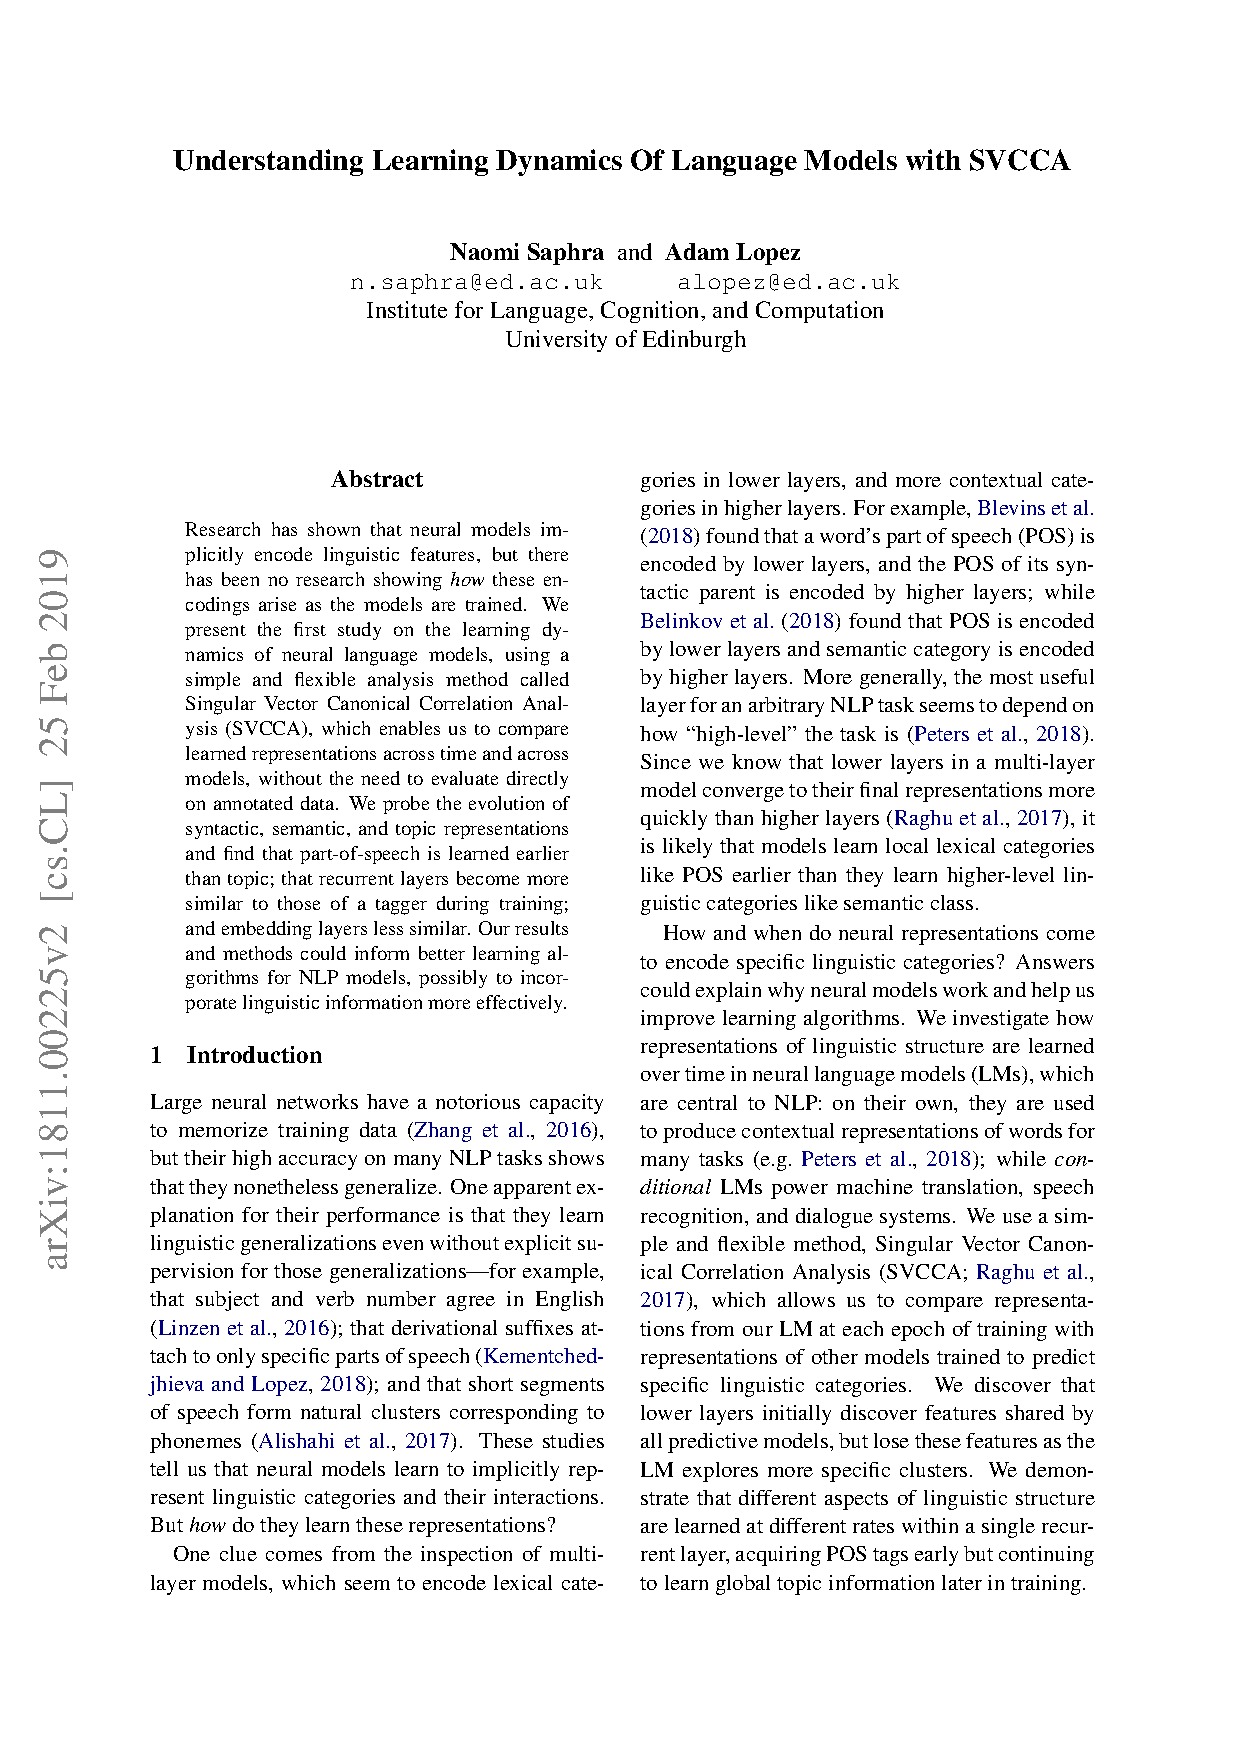
\includepdf[pages=-,pagecommand={}]{svcca/chapter.pdf}

\section{Comments on the paper}

In addition to the insights we gain from observing the time course of training, the model similarity method we use provides some intriguing insights even without considering the time dimension. When looking at input tagging instead of next-tag prediction, we find that more granular tagging produces representations that are more similar to LM representations (e.g., a model predicting simple Universal Dependencies POS tags produces more LM-like representations than a model predicting more granular PTB POS tags). This result suggests that complex tag information is retained from input words, but the structure ultimately encoded in predictions does not resemble the linguistic ontologies. We also see that input structure itself is retained, even given random target labels, based on the high baseline similarity between the language model and randomized (that is, with \textit{memorized} outputs) taggers. Results like this suggest \textit{general} properties of the LSTM, and possibly further of neural networks, in their reliance on input structure independent of output.

These insights suggest the possibility of using similarity as a general probing method, outside of training dynamics experiments--and indeed, since the publication of this paper, representational similarity methods have been widely applied in NLP. \citet{chrupala_correlating_2019} and \citet{chrupala_symbolic_2019} both explored the correlations between different vector and symbolic representations using Representational Similarity Analysis. \citet{movva_dissecting_2020} and \citet{bau_identifying_2018} used neuron-level similarity to compare models. \citet{voita_bottom-up_2019} looked at the similarity between different layers of a Transformer model using a different variant on CCA, PWCCA. \citet{singh_bert_2019}, meanwhile, compared representations in different languages using unadorned CCA, and \citet{hsu_zero_2019} used SVCCA as in our paper. \citet{chung_similarity_2020} and \citet{wu_similarity_2020} both surveyed a variety of similarity techniques, with \citet{wu_similarity_2020} validating one of the assumptions behind our method by confirming that similar architectures produced similar representations. Note that nearly all of these works postdate the work in this chapter, and almost all of them cite it.

While in general, models are more accurate when they are more similar to the same architecture trained with different seeds \citep{raghu_svcca:_2017}, it is yet to be seen whether high similarity \textit{across tasks} (e.g., LM compared to a tagging task as in this paper) indicates higher LM performance. If so, it would be interesting to see \textit{which tasks}. Can we glean information about LM performance from similarity to representations for all tasks, or only for those that involve a closer distance of dependencies (POS) or farther (topic)? This is an essential result to confirm that similarity analysis avoids one of the flaws of diagnostic classifiers: a lack of correlation between model accuracy and probe accuracy.

It is worth noting that there is no theoretical reason establishing that modules should have high similarity scores, even if they are the same type of module and situated with a similar environment in the pipeline of a model, but in practice \citep{chung_similarity_2020,raghu_svcca:_2017,morcos_insights_2018} this does seem to be the case. Therefore, although CCA yields specifically a \textit{linear} similarity, it is distinct from the common use of linear functions as probing models in that there is a clear empirical justification for the assumption that two representations  will be linearly similar, if they are accomplishing the same function (such as  representing POS as a recurrent module feeding into a softmax layer).

\subsection{Generalizing to Attentional Models}

The methods of this paper could be straightforwardly applied to any Transformer-based LM, including masked LMs rather than autoregressive. In order to do so, one would substitute the desired tag for the word being predicted and apply SVCCA to the activation vectors produced by, e.g., the feedforward layers of each Transformer module. In addition, similarity of the attention distributions used by models predicting a tag vs. a word could be measured through Shannon- or KL-divergence.

% \chapter{Cross-lingual Transfer in Sentiment ANalysis}
\label{chapter:multilingual_sentiment_analysis_pt2}


% \chapter{Beyond Words: The Development of Feature Sparsity} \label{chapter:sparsity}

\epigraph{``In this box are all the words I know,'' he said. ``Most of them you will never need, some you will use constantly, but with them you may ask all the questions which have never been answered and answer all the questions which have never been asked.''
}{Norton Juster, \textit{The Phantom Tollbooth}}
% \epigraph{``It will take years to collect all those sounds again,'' she sobbed, ``and even longer to put them back in proper order. But it's all my fault. For you can't improve sound by having only silence. The problem is to use each at the proper time.''}{Norton Juster, \textit{The Phantom Tollbooth}}

In Chapters \ref{chapter:svcca} and \ref{chapter:interdependence}, we explored the temporal dynamics of models acquiring linguistic structure as training progresses. Here we turn to investigate more abstract properties of representations and how they evolve. In particular, the following work explores how \textbf{feature sparsity} naturally emerges in LMs during training. 

Rather than consider the gradual development of hierarchical syntactic structure, we observe the dispersal or concentration (i.e., sparsity) of intermediate vector representations as a simple function of the frequency and predictability of each word. We better characterize the relationship between word frequency and the distribution of its ``storage'' in a model. The time dimension is essential to understanding the contributing factors to sparsity, because the model is more exposed to a word the longer it trains for, as well as in response to the word's corpus frequency. 

As well as providing consideration of this crucial confounding factor between word frequency and a model's exposure to a word, viewing the time course of training again offers additional insights. We see how gradients responding to a word become sparser--meaning salient information is localized to a few neurons--as a network is exposed more to that word. This validates work that considers individual neurons rather than entire subspaces \citep{hennigen_intrinsic_2020,durrani_analyzing_2020,dalvi_what_2018}. We see that LSTM layers quickly correlate word frequency and sparsity, before the embedding layer surpasses the LSTMs in developing this correlation. The patterns we observe are, as in Chapter~\ref{chapter:svcca}'s discussion of the Information Bottleneck Hypothesis, possibly linked to a memorize/compress phase shift. 


\paragraph*{Publication Status } This work was published in the Identifying and Understanding Deep Learning Phenomena Workshop at ICML 2019.


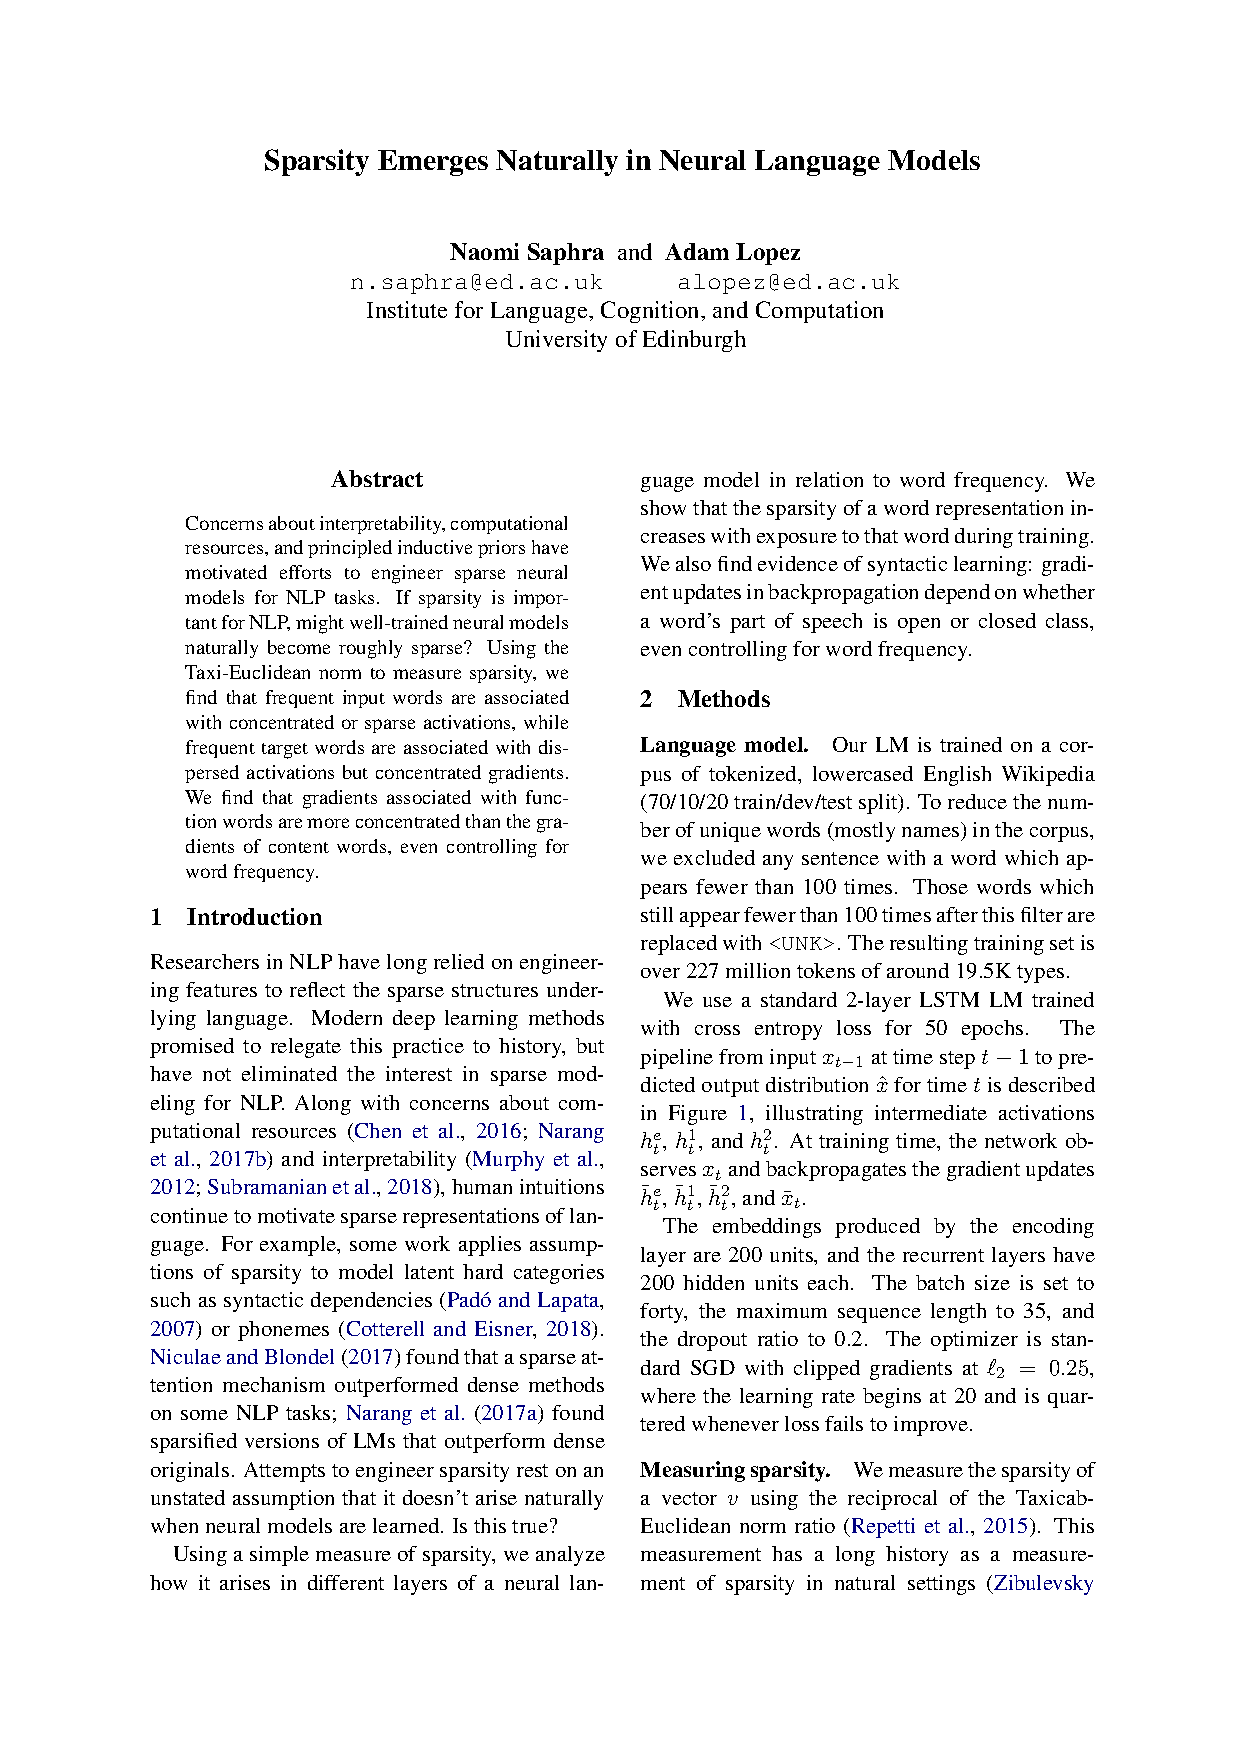
\includepdf[pages=-,pagecommand={}]{sparsity/chapter.pdf}

\section{Comments on the Paper}

In this paper, we have investigated the sparsity of activations and, using the same sparsity metric applied to gradients, observed how localized change is across neurons. 

\subsection{Localization of Changes}

The local loss surface revealed by gradients is not the only way of viewing change across neurons. Because the optimizer does not follow this surface perfectly, and the training data is not the only way of viewing change in error, we may want to investigate change in each neuron through \textbf{Loss Change Allocation} (LCA)~\citep{lan_lca:_2019}.

\subsubsection{Loss Change Allocation} \label{sec:lca}

LCA is a method that does not look directly at the gradient with respect to training error, but instead allocates responsibility for \textit{actual} error change after a training step.

If we consider the loss function over a training set $L(\theta_t)$ with the parameters at timestep~$t$, LCA is based on a first order Taylor approximation of the path between two timesteps:
\begin{align}
    L(\theta_{t+1}) - L(\theta_t) &= \int_{\theta_t}^{\theta_{t+1}} <\nabla_{\theta} L(\theta_t), d \theta>\\
    & \approx < \nabla_\theta L(\theta_t), \theta_{t+1} - \theta_t>
\end{align}

This dot product can be reformulated into an element-wise operation, such that we can consider the individual parameters that contribute to this change in loss. We therefore define the LCA allocated to parameter unit $\theta^{(i)}$ like so:
\begin{equation}
    \sum_{i=0}^{K-1} A_{t,i} = \sum_{i=0}^{K-1} (\nabla_{\theta} L(\theta_t))^{(i)} (\theta_{t+1}^{(i)} - \theta_t^{(i)})
\end{equation}
This way, we could consider whether following the gradient in a particular direction actually leads to a particular unit improving or damaging performance when considered in combination with the other changes made during that timestep. 

Using LCA, \citet{lan_lca:_2019} found that only a little over half of parameters actually help improve performance in their changes at any given time step, with some entire layers moving against the gradient in a particular timestep and damaging performance. Because all layers tend to move in synchrony, they hypothesize that these damaging layers lag behind others while they oscillate back and forth over valleys in the optimization landscape, therefore moving against the overall gradient motion. These dynamics calls into question a simplistic view of the training process through the lens of the gradient landscape itself. Even from timestep to timestep, the movement of parameters along the gradient does not translate directly to improvement in the training objective.

\subsection{Generalizing to Attentional Models}

Current Transformer models provide new motivations and methods for considering sparsity during the forward pass through a neural network. Attention distributions can be easily measured in terms of their entropy, which offers additional information about how localized word importance itself might be, as it gives a view of how sparse \textit{attention} naturally is across words.

% \chapter{Conclusion}\label{chapter:conclusion}

%“For every subtle and complicated question, there is a perfectly simple and straightforward answer, which is wrong. —H.L. Mencken”
In this section I will condense the takeaways from my work, then expand them into the questions they pose. I'll discuss implications for future work, and do a bit more theorising than in each individual conclusion, made possible by the aggregation of all the works. I will also relate my work to the present day mania for Large Language models (LLMs), generative AI, and scaling.

This body of work has focused on \textbf{measurement of fairness}, and on then, with respect to those measurements, on \textbf{analysis of monolingual and cross-lingual transfer}, and analysis of \textbf{dense retrievers}. We contributing to enriching the understanding of fairness within a multi-part system, which was previously very poorly understood. This poverty was much more marked at the commencement of this work than today, but does still persist. Fairness and interpretability research have grown, but so has the field as a whole.\footnote{Fairness work has grown exponentially, but so have ACL and NeurIPS, both with about 40-50\% growth in submissions year over year, \url{https://aclweb.org/aclwiki/Conference_acceptance_rates} and \url{https://medium.com/criteo-engineering/neurips-2020-comprehensive-analysis-of-authors-organizations-and-countries-a1b55a08132e})} The scale and speed of productionisation still far outstrips understanding. 

In Part~\ref{part:measurement} I first examined the dominant method of bias evaluation in language models, based on embedding geometry and cosine similarity, found it to have poor predictive validity. I advocated for measuring bias downstream. 
I next found an alternative upstream measure in information theoretic probing of demographics. I caveat that it shows though only \textit{potential} for social bias downstream, a potential that may or may not be realised depending on classifier training. The full system is still needed to see the full picture.

In Part~\ref{part:crosslingual}, I examined monolingual and cross-lingual transfer in the setting of sentiment classification, in five languages, and found that both settings changed fairness outcomes. Monolingual transfer generally improved fairness despite the introduction of new data scraped from the depths of Common Crawl. I attributed this to increased stability in model decisions from the additional data: where stability is defined as not just less errors under the counterfactual, but smaller magnitude ones. Multilingual transfer, however, often worsened fairness outcomes, despite using more data than monolingual transfer. This may not contradict the previous result, as there are less parameters per language, such that even with regard to performance multilingual transfer models are not more stable than monolingual transfer models. The reasons for this difference are left to future work. 

In Part~\ref{part:generation}, I examined dense retrieval models, using the tools and research questions accumulated in Parts~\ref{part:measurement} and \ref{part:crosslingual}. I found that random initialisation and random data shuffle play a much larger role than previously thought. This challenges the standard practice of using only one random seed for research, which was then common and is now ubiquitous in the age of LLMs, where training one model takes over 400,000 kWh \citep{luccioni_bloom_carbon}, or the same amount of energy to make 14 million cups of tea, approximately the same amount that is drunk in Scotland daily.\footnote{It takes about 336000 joules to raise 1 liter (4 cups of tea) of water to a boil, which is equivalent to 0.116 kWh assuming an electric kettle at 80\% efficiency. This makes an LLM equivalent to approximately 13,714,286 cups of tea. The UK drinks on average 3 cups of tea per day, and the population of Scotland is 5.4 million today.} No one does this twenty five times, as I did here. In this work I also found a case where information theoretic probing was \textit{not} predictive of gender bias in retrievers, because the bias was caused by other factors beyond the model representation itself. 

The combined work in this thesis repeatedly shows how little it makes sense to make choices or come to conclusions about fairness without understanding and simulating the entire system. 

Each individual work raised as many questions as it answered, which have not yet been answered by other analytical work. These questions are significant in both size and importance and would be valuable extensions to the understanding of the field, even in the era of LLMs. For both works in Part~\ref{part:measurement} the question remains: what about generative models?  What is the relationship between upstream language model metrics and downstream bias in generation, as opposed to in classification? The objective in generation is more similar to that of pre-training, so the story may be different. Chapter~\ref{chapter:gender_bias_probing} showed that whether bias was realised was a property of both the language model and the classifier, so what if there's no classifier? 
But to answer that question, there has to be a way to measure bias in generation, which the field has by no means settled on, as we discuss in \S\ref{sec:measuring_fairness}. 

In Part~\ref{part:measurement} in classification, I used observational studies to determine allocational bias by measuring whether the error rates across populations that differ with respect to a demographic variable were equal (male group vs. female group, etc). In Part~\ref{part:crosslingual} I used interventional studies that measured whether change in a demographic variable changed predictions, when the predictions should be equal. Both of these measurements require a notion of equality -- which is very easy with a discrete label space or ordinal values. The same type of study could be set up for generative models: instead of classifying resumes, a model could write summaries of resumes with a recommendation to proceed or not, which is then read by a human.\footnote{This is what is happening in practice with generative AI now.} We can make the same assertion, that if we change the gender or race on the resume, the summary should not materially change. But what is a \textbf{material change}? In principle, it is a change that is large enough to cause the summary to be less accurate. Or to be equivalently accurate but to affect a human's opinion positively or negatively. Probably we want to know both for different reasons. How do we measure this? 

The little previous work on this raises just as many questions. \citet{vig_causal} consider social bias in generation to be the relative probability of different gendered pronouns along with stereotypical professions like \textit{doctor} and \textit{nurse}. But how would that be extended to different grammatical systems, like Turkish, which has no gendered pronouns? What about different demographic biases that aren't encoded the way gender is? There is far less research about those \citep{}, but they are no less important from the viewpoint of ethics or of law. 
%Even with those worked out, this measure is so zoomed in that, while it matters, it's hard to see what scope of bias problems it can and cannot represent. 
%BELOW IS REDUNDANT
%\citep{sheng-etal-2019} use \textit{regard} of the demographic that a generation is about, which is generalisable as a notion, but not in practice when operationalising: they train one classifier, which is available in English only, for three binaries (male/female, white/black, and gay/straight) and has never been updated. 
\citet{BOLD}, which is used in most LLM works today (e.g. \citep{llama2,jiang2024mixtral}) create a dataset where they use gender term frequency and regard, in combination with sentiment and toxicity, to try to overcome the issues of each. 
%Plenty of harmful stereotypes carry positive sentiment [example] and lots of social bias doesn't manifest via differences in toxicity [example. 
More essential measurement groundwork has to be done for generation before we can begin to determine whether these metrics are predictable from upstream metrics.

The second work in that section, Chapter~\ref{chapter:gender_bias_probing}, raises the question: what about beyond gender? Most work in this thesis by design looks as bias beyond gender (\ref{chapter:intrinsic_bias_metrics}, \ref{chapter:multilingual_sentiment_analysis}, and \ref{chapter:multilingual_sentiment_analysis_pt2} all include some notion of race or country of origin) but this one,  which proposes a new metric, looks only at gender (partly for lack of suitable datasets beyond it). But gender is encoded very differently in language than other demographic features, so it could reasonably have a different way it operates in model representations and social bias. In English, which weakly marks gender, and other languages with stronger gender agreement, gender is clearly important to represent for correct grammar and language reconstruction from a noising objective \citep{}. But race and country of origin are not as strong signals: it is not easy to determine these save from specific words like names (and even then the signal is not perfect at all, unlike with pronouns). How does this difference in encoded information affect the relationship between language models and downstream bias?

In Chapter~\ref{chapter:multilingual_sentiment_analysis} we found that there was less bias in aggregate in monolingual transfer, and more reasonable patterns of bias (less dramatic changes in sentiment score), but what about tracing individual examples through from pre-training? Could we track a specific negative stereotype in pre-training and see if it can affect decisions later? Extending to the work in Chapter~\ref{chapter:multilingual_sentiment_analysis_pt2}, could we extend tracing individual biases into multiple languages? Almost all bias research is done on aggregate information, and we extended our focus to be on patterns of bias, but we stopped short of doing fine-grained analysis. A more granular analysis would be valuable. We've spent this thesis tracing how fairness persists and travels through a system at a macro level, but we could extend this to a micro level. Such research would not even be bias specific; for there isn't concrete knowledge yet of how \textit{any} information travels between different training stages of models (of which there are increasingly many in the age of LLMs).

In Chapter~\ref{sec:fairness_as_other_fields}, I introduced the notion of fairness as a generalisation error vs. as a learnt dataset artifact (whether an artifact from spurious correlation or a historical bias). A deeper investigation into this could help enlighten why racial bias can increase with cross-lingual transfer. Is it really compounding biases (stereotypes) or could it be a generalisation error? One of these types of bias would have much less certainty than the other. Can an investigation into model uncertainty help illuminate which of these cases is involved in any measurements we observe?

Part~\ref{part:generation} shares the question of biases beyond gender from Chapter \ref{chapter:gender_bias_probing}, as it is also solely gender focused. It also raises many questions that have particular importance to fairness but are also general to our understanding of our systems as a whole. Why is random seed initialisation so important for bias and for generalisation? Why is it possible for a couple of seeds to \textit{just not work at all}, never mind fairness? Some of the anistropy of the representations from earlier training stages seems potentially predictive of later behaviour. Can we understand this well enough to utilise it? If so we could be able to actively encourage model training that is less prone to shortcutting. 

Now I want to bring this into current industry practice and zeitgeist. I do this partly because I've spent the better part of the last year working full-time on fairness at an LLM company. And partly because, in reviewing my PhD work, I don't want to ignore the sea change in NLP research that's taken place over the past year. I am not someone for whom `\textit{scaling is a way of life}'\footnote{This light shade given by Tatsunori Hashimoto when questioned about it at GenBench at EMNLP 2023.}, but it would be disingenuous, in a field intended to improve people's lives, to not speak about how my work relates to current research, current discourse, and current practice. This thesis was initially inspired by a sea change that I saw happening six years ago, after all. 

This work was all done on models three orders of magnitude smaller than the ones that I deal with in my work today. 

This does not matter at all. No conclusions in this thesis were model specific. If some architecture arises to replace neural embeddings, LSTMs, and Transformers which bears no genetic link to it, then they may no longer hold. But until that day (which will be very exciting, it would be nice to move on) the defferences between the models I use at work today and the models in this thesis are: 1) scale 2) a veneer of RLHF (Reinforcement Learning from Human Feedback \citep{} 3) instruction tuning \citep{} and 4) more math, logic, and code in both pretraining and fine-tuning than is usually present in NLP tasks (though some non-trivial amount will of course be present in CommonCrawl, which does drive the models in this thesis). None of these differences affect my conclusions. 

In my first rebuttal for \ref{chapter:intrinsic_bias_metrics}, temporally as well as sequentially the first paper in this thesis, Adam told me how to rebut one of the reviewers asking `But have you tried this on {\tt Newest Model Architecture}' (which in this case was BERT). He instructed me to turn that into a the question, `Is there any reason to expect that architecture would behave differently? Otherwise, they're just saying \textit{New thing is Magic}'. There is no reason to believe and of the four recent innovations change any of the discovered fairness behaviours here.

The replication and extension of my work in \ref{chapter:intrinsic_bias_metrics} by \citet{cao-etal-2022-intrinsic} did use BERT, and 18 other transformer architectures of varying sizes, and came to the same conclusions. 

We've seen the same bias amplification affects at scale \citep{} that we saw in \citet{zhao-etal-2017-men}. Current research shows that the RLHF (and family of alignment algorithms) predominantly affects style and structure of response, rather than content \citep{min-etal-2022-rethinking,  lin2023unlocking} and can be trivially changed and doesn't affect true fairness behaviour \citep{qi2023finetuning} and that all information is learnt at earlier stages, predominantly pretraining \citep{zhou2023lima}.
So the addition of an RLHF step to current SOTA models does not change any of these conclusions.

There is one salient change that will matter. Language models are essentially trained to compress and then reconstruct the data they were trained on, and this lossy compression has become less lossy as an effect of scaling \citep{karamolegkou-etal-2023-copyright}. This could change fairness outcomes, though will it help or will it harm? This depends somewhat on whether the source of the unfairness is a dataset artifact or a generalisation error (\S \ref{sec:fairness_as_other_fields}) in that overall increased memorisation is likely to exacerbate the learning of artifacts, but improve generalisation (though generalisation ability is difficult to test in the current era of closed language models and unknown pretraining and fine-tuning data). This effect from scaling won't change the measurements of mechanisms of bias transfer, which are the subject of this thesis, but they do lend weight to the need for more work on disentangling sources of bias and looking at the effects of increased memorisation from overparameterisation. 

When I started this thesis I focused on validating metrics, not because of a dedication to evaluation; I had grand plans for applying my ideas to cross-lingual bias mitigation. But I'd seen unvalidated assumptions in the standard metrics of the field, and it made me nervous about using those metrics in my own work. I didn't want to stake my PhD research and journey on a metric that I didn't believe in and find out 1.5 years in. But now that I work in a deployed product, I focus predominantly on evaluation. I do some fine-tuning and synthetic data creation, but about half my energy is spent on evaluation. Because good evaluation was \textit{always very hard} and the rise of generative AI has only made it harder. [do I need to say more here] And I can only throw darts at a wall if I know when they've hit something useful, and that's the hard part, not the dart throwing. 

There is some irony in how my first fairness work showed that you cannot do upstream social bias mitigation, and then I took a job where, to succeed, I am supposed to do just that. And where in practice, I need to, since education about NLP systems is not good enough that many of the people deploying language models have the knowledge or resources to do bias mitigation themselves. So, I use the tools and the ways of thinking and discoveries that I made over the course of this thesis to evaluate and analyse and create bounds for what types of bias could occur in different reasonable settings, and then make this information public, so that deployers know and can work around it. 

But this is still not satisfying enough. I do not think we will ever get to a point in which we rely on one single large pretrained model for thousands of use cases and can predict bias effects downstream for anything but the most common ones. All of this research has progressively taught me that I need to consider the entire NLP system in my measurements for bias: the pretraining, the fine-tuning, the task, the inputs, the corpus that a model can query. The limit case of this it that I need to consider the user interface, the users themselves, the societal power structures within which the NLP system is embedded. And I do think, at some stage, these do need to be part of the experiment conditions and considerations. We cannot consider the harmful effects of QA systems providing false information in absence of how it is displayed in a UI, and how much that UI encourages trust or overreliance \citep{} and bias research cannot consider stereotypes in absence of the power structures that make them harmful \citep{blodgett-etal-2021-stereotyping}. No more can most NLP systems be considered without these things, which all together make it increasingly challenging/impossible to predict all of these things at an upstream stage. 

But we can get to a point where we understand better what choices we've made in the lifecycle of an NLP system tend to make things worse or better, and why. With that, we can better predict bias potential in new systems and then with that knowledge set up evaluations and mitigation methods. So that we can take a set of facts about a model, and then generalise from it. %like humans do





% NOTES:
% The role of fairness research is the understanding that industry doesn't have time to do but that can still have hope of being applied in practice of having bearing on a real world situation -- this is a characteristic of the field since it is necessarily grounded in real humans and their lives.


%We are building out the picture of the full ecosystem of what can matter over the course of the thesis




% WHAT else can I bring in about science about goodharts law about things I've learnt about doing this all in practice?


%%% Outline what I want to cover in the discussion

\bibliographystyle{apalike}
\bibliography{bibl}

\appendix

\end{document}
